\chapter{Trabajo y Energía}

\textit{``El movimiento es un modo de ser que resulta necesariamente de la materia; ésta se mueve por su propia energía; sus 
movimientos se deben a las fuerzas que le son inherentes.''}\textbf{Barón de Holbach}\vspace{1.0 cm}

El concepto de energía (\textbf{E}) es uno de los más utilizados y destacados en esta ciencia. En este Universo la energía juega 
un papel muy importante, es aquella encargada del movimiento de los cuerpos y que los procesos naturales sean posibles.

\begin{tcolorbox}
La energía es la capacidad que poseen los cuerpos para poder efectuar un trabajo (movimiento) o de lograr alguna transformación.  
\end{tcolorbox}

Según la forma o el sistema físico en que se manifiesta, se consideran diferentes formas de energía: térmica, mecánica, 
eléctrica, 
química, electromagnética, nuclear, luminosa, etc. En cuanto a su unidad de medida es el "JOULE" ó "JULIO", que se denota 
simplemente como \textbf{J}.\\

Aunque la energía puede cambiar de forma en los procesos de conversión energética, la cantidad de energía se mantiene constante 
conforme con el \textbf{principio de conservación de la energía} que establece:

\begin{tcolorbox}
``La energía no se crea ni se destruye, sólo se transforma''. 
\end{tcolorbox}

Por consiguiente, la energía total de un sistema aislado se mantiene constante y en el universo no puede existir creación o 
desaparición de energía, sino transferencia de un sistema a otro o transformación de energía de una forma a otra, es en otras 
palabras, la energía es una invariante física. Así en un sistema aislado se tendrá que la energía total de cuyo sistema es el 
mismo, es decir:

\begin{equation}
E_{inicio} = E_{final}
\end{equation}

En este momento nos referiremos específicamente a la energía mecánica ($E_m$) la cual es aquella relacionada con el fenómeno del 
movimiento, y así está energía se la puede visualizar como la suma de la energía cinética ($E_c$), la energía potencial 
gravitatoria ($E_p$) y la energía potencial elástica ($E_k$), así inicialmente:

\begin{equation}
E_m = E_c + E_p + E_k \quad [J]
\end{equation} 

\section{Energía cinética:}

Esta energía es la que tiene un cuerpo movimiento por el simple hecho de que tiene una velocidad diferente de cero. Por tanto la 
energía que tiene un cuerpo de masa $m$ cuya velocidad $v$ es:

\begin{equation}
E_c = \frac{1}{2}mv^2
\end{equation}

\section{Energía potencial gravitatoria:}

Está energía está asociada a la posición que tienen los cuerpos, y no a su movimiento. Se define como aquella que poseen los 
cuerpos por el hecho de encontrarse en una determinada posición en un campo de fuerzas.\\

Un concepto más acertado es el siguiente:

\begin{tcolorbox}
La energía potencial gravitatoria. de una masa en un punto del espacio es el trabajo que realiza en un campo gravitatorio para 
trasladar la masa desde dicho punto hasta el infinito. 
\end{tcolorbox}

Es decir, está energía es la que posee un cuerpo por el hecho de encontrarse bajo la acción de la gravedad. Su valor, para el 
caso 
de alturas pequeñas sobre la superficie terrestre, viene dado por:

\begin{equation}
E_p = mgh
\end{equation}

donde la $h$ es la altura del cuerpo con respecto al suelo.

\section{Energía Potencial Elástica:}

Esta energía es la que se almacena o se libera cuando un resorte es comprimido o estirado, esta energía depende del material del 
resorte como también de la variacción de su longitud al ser manipulado.\\

Todo resorte tiene una constante elástica $k$ llamada constante de elásticidad del resorte y está relacionado con la energía 
potencial elástica ($E_k$) como:

\begin{equation}
E_k = \frac{1}{2}k\Delta x^2
\end{equation}

donde $\Delta x$ es la longitud comprimida o alargada el resorte por una fuerza. Un concepto más acertado de está energía es el 
trabajo realizado por una fuerza al comprimir o alargar un resorte.

Se ha mencionado el término de trabajo, por lo cual es pertinente conocer el significado físico de ese término.

\section{Trabajo mecánico:}

El trabajo mecánico es la capacidad de una fuerza para desplazar un cuerpo una cierta distancia. Es decir, es esa energía 
necesaria para poder mover a ese cuerpo una distancia mediante una fuerza.\\

\begin{figure}[ht]
 \centering
 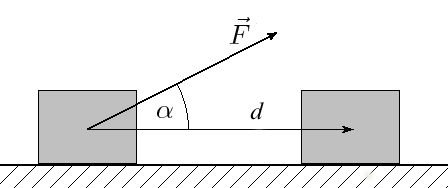
\includegraphics[scale=0.5]{images/trabajo.png}
 % cinematica.png: 0x0 px, 300dpi, 0.00x0.00 cm, bb=
 \caption{Ilustración del trabajo mecánico.}\label{tmec}
\end{figure}

El trabajo es una magnitud física escalar que se representa con la letra $W$ y se expresa en unidades de energía (\textbf{J}) en 
el Sistema Internacional de Unidades. Para el cálculo del trabajo sólo se tiene en cuenta la componente de la fuerza que actúa en 
la dirección de desplazamiento del cuerpo, por lo que el trabajo es una magnitud escalar. De este modo el trabajo se computa así:

\begin{equation}
W = \vec{F}\cdot\vec{\Delta r}\quad [J]
\end{equation}

donde se observa que el trabajo mecánico es el producto escalar entre la fuerza $\vec{F}$ y el desplazamiento $\Delta \vec{r}$ 
que 
realiza el cuerpo bajo la influencia de $\vec{F}$.\\

El trabajo mecánico puede tener dos signos: uno positivo y otro negativo. El signo positivo es cuando la fuerza aplicada va en el 
mismo sentido del movimiento, pero es negativo cuando va en contra del movimiento, ya que el trabajo mecánico es:

\begin{equation}
W = F\Delta r cos(\theta)
\end{equation}
 
siendo el $\theta$ el ángulo entre la fuerza $\vec{F}$ y el desplazamiento $\Delta \vec{r}$. También, existe el caso cuando el 
trabajo es nulo que correspondería cuando la fuerza y el desplazamiento son perpendiculares entre sí.
  
\section{Potencia:}  

La potencia se puede entender como la rapidez con la que se efectúa trabajo y se define como el trabajo realizado por unidad de 
tiempo. La potencia mecánica se simboliza con la letra P

\begin{equation}
P = \frac{W}{\Delta t}\quad [W]
\end{equation}

También la potencia la podemos expresar en término de la velocidad, para cuando la fuerza es constante

\begin{equation}
P = Fv
\end{equation}

Las unidad de medida para la potencia en el S.I son el Watts ($W$), el cual se define como $Joule/s$.

\section{Problemas de trabajo y energía}

\begin{enumerate}

\item Un hombre sube por las escaleras de un edificio llevando a cuestas una lavadora que pesa 500 N, y cuando llega al octavo 
piso, se había dado cuenta que se ha equivocado de edificio, y regresa a la planta baja. Si el octavo piso esta a 20 metros de 
altura, ¿cuál fue el trabajo realizado por el hombre durante su recorrido?

\item Se suelta un bloque de masa de 10 kg desde lo alto de un plano inclinado que forma un ángulo de $30^\circ$ con la
horizontal y de longitud 50 cm. El bloque choca contra un resorte horizontal ideal y lo deforma 10 cm en la parte baja del plano 
inclinado. Conociendo que el coeficiente de rozamiento entre el plano inclinado y el bloque es 0.3; determine la constante 
elástica del resorte.

\item Un pedazo de plastilina, de 40 g de masa, se mueve con velocidad de 100 m/s y choca, quedando incrustada, en un bloque de 
madera de 1 kg de masa que está en reposo. El bloque está unido a un muelle que se contrae 20 cm. Si no hay rozamiento entre 
el suelo y el bloque, determina el periodo de oscilación del movimiento vibratorio generado.

\item Una maceta cae de un balcón a una velocidad de 9,81m/s adquiriendo una energía cinética de 324J, ¿cuál es su masa?  

\item Una persona transporta sobre sus hombros un bulto de 25 kg con el que recorre 20 m. Determina el trabajo realizado para 
soportarlo. 

\item Un automóvil de 1.500 kg lleva una velocidad de 120 km/h por una carretera horizontal. En un determinado momento ve un 
obstáculo y frena hasta pararse. Calcula el trabajo realizado.

\item Un automóvil de 1.000 kg tarda 8 segundos en alcanzar la velocidad de 72 km/h.¿Qué potencia desarrolla el motor sabiendo 
que 
la fuerza de rozamiento es equivalente a la décima parte del peso? 

\item Se tiene un plano inclinado cuya longitud es 15 m y cuya base es 9 m. ¿Con qué velocidad y con qué energía cinética  
llegará 
a su extremo inferior un cuerpo de 60 Kg que partió del extremo superior con una velocidad de 2 m/s? 

\item  Si la masa de un cuerpo se duplica y su velocidad se reduce a la cuarta parte, ¿cómo cambia su cantidad de energía 
cinética?

\item  Una pelota de fútbol de 550 g de masa adquiere una velocidad de 70 m/s mediante un puntapié de 0,2 s de duración, ¿cuál 
es el trabajo mecánico realizado por la fuerza ? 

\item  Sobre un cuerpo de 10 kg de masa actúa una fuerza de 100N que forma un ángulo de 30º con la horizontal que hace que se 
desplace 5 m. Si el coeficiente de rozamiento entre el cuerpo y el suelo es 0,2, calcula el trabajo realizado por la normal. 

\item Calcule la potencia realizado por un motor de un ascensor de 300 kg que se eleva a una velocidad 0.5 m/s.

\item Un paquete es lanzado por un plano inclinado $20^\circ$ con la horizontal con una velocidad de 8m/s en un punto A del 
plano. Llega a un punto B situado 7 m más arriba de A y se detiene. ¿Cuál es el coeficiente de fricción entre el paquete y el
plano inclinado?

\item Un cuerpo de 1,5 kg de masa cae desde 60 m. Determinar la energía potencial y cinética a 15 metros antes de topar el piso.

\item  Un motor eléctrico realiza trabajo sobre un compresor a un ritmo de 1.5 KW. ¿Cuánto trabajo ha realizado en un mes si el 
compresor funciona ininterrumpidamente?

\item Una fuerza de 150 N paralela a un plano inclinado de ángulo $30^\circ$ actúa sobre un cuerpo de masa 10 Kg. Si el cuerpo 
asciende 5 m por el plano inclinado y μ= 0,2. Calcular la energía perdida como calor.

\item  Un cuerpo 4 kg cae desde 2,3 m de altura sobre un resorte cuya constante es 200 N/m. Calcular la velocidad del cuerpo 
cuando el resorte se ha comprimido 2.5 cm.

\item Se deja caer sobre un muelle en posición vertical una masa de 0.5 kg desde 1 m de altura. El muelle tiene una longitud de 
0.5 m y una constante de 100 N/m. Calcular la longitud h del muelle cuando está comprimido al máximo.

\begin{figure}[h]
 \centering
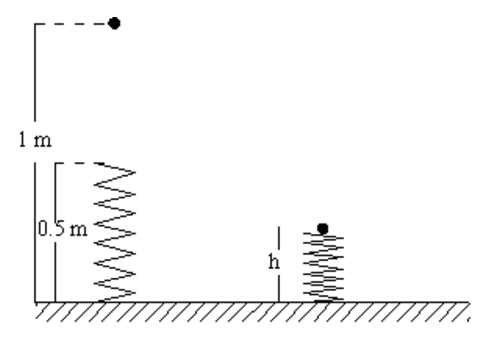
\includegraphics[width=4.0cm,height=3.0cm]{images/energia.eps}
\end{figure}

\item Desde la parte más baja de un plano inclinado, sube un bloque hasta detenerse en la parte más alta del mismo plano. Si la 
energııa mecánica total del bloque en la parte inferior y la superior es de 100J y 70 J, respectivamente, determine el 
coeficiente de rozamiento entre el bloque y el plano.

\item Se lanza una pelota desde 2m de altura. En el segundo rebote la altura que alcanza es 0.35 m. ¿Qué porcentaje de energía 
pierde cada vez que rebota?

\item Se suelta un bloque de masa de 10 kg desde lo alto de un plano inclinado que forma un ángulo de $30^\circ$ con la 
horizontal y de longitud 50 cm. El bloque choca contra un resorte horizontal ideal y lo deforma 10 cm en la parte baja del plano 
inclinado. Conociendo que el coeficiente de rozamiento entre el plano inclinado y el bloque es 0.3; determine la constante 
elástica del resorte.

\item  Un paquete es lanzado por un plano inclinado $20^\circ$ con la horizontal con una velocidad de 8m/s en un punto A del 
plano. Llega a un punto B situado 7 m más arriba de A y se detiene. ¿Cuál es el coeficiente de fricción entre el paquete y el 
plano inclinado?

\item El quarterback de un equipo de fútbol americano lanza el balón (435 gramos de masa) con una velocidad de 18 m/s y ángulo de 
$50^\circ$ respecto a la dirección horizontal. Debido a la fricción del aire, el balón cae al suelo 0,5 metros antes de lo que 
habría alcanzado en ausencia de la fricción. Con base en lo mencionado anteriormente y suponiendo una fricción constante en la 
dirección de horizontal, determine: a) La aceleración que imparte la fricción del aire al balón, b) el trabajo realizado por 
dicha fricción sobre el balón, y c) la energía cinética que el balón pierde debido a esta fricción. 


\end{enumerate}
